\documentclass[11pt,a4paper]{article}
    \usepackage{listings}
    \usepackage{hyperref}
    \usepackage{graphicx}
    \usepackage{float}
    \usepackage{placeins}
    \usepackage{subcaption}
    \usepackage{cleveref}
    \usepackage{booktabs}
    
    
    \newcommand{\acomment}[1]{{\bf{\color{blue}{{[Aman: #1]}}}}}
    \newcommand{\scomment}[1]{{\bf{\color{blue}{{[Suyash: #1]}}}}}
    
    \hypersetup{
    colorlinks=true,
    allcolors=blue,
    }
    
    \usepackage{geometry}
    \geometry{
    a4paper,
    % left=25mm,
    % right=25mm,
    top=30mm,
    % bottom=30mm,
    }
    
    \title{Action Report 2017-18}
    \author{Software Development Club, IIT Delhi}
    
    \begin{document}
    
    \maketitle
    \section{Overview}
    DevClub is the software development club of IIT Delhi with an aim to foster
    software development culture in the institute. It provides a platform for
    students who are passionate about technology to explore the field. The club
    has two main objectives. The first goal is to form a body of
    passionate students, who would use their skills to develop solutions for real
    problems at IIT Delhi and beyond. The second goal is to spread the knowledge that they
    acquire to the uninitiated, so that more and more people take part in
    development.\\
    
    
    Before DevClub, most of the students were uninterested in program design. This technical knowledge is not usually imparted in our courses and people didn't take the extra effort to learn it on their own. Most of the students in their first year went the extra mile to learn music, dance, sports from their respective clubs. The result was that no one was trying to learn development and those handful students who were at least a little bit interested lost their passion because they had no support other than the internet. After seeing all this, it was decided that the only way to improve the technical aptitude of the institute was to form a club where ardent students would work together to learn new technologies, develop software which had real applications and spread their knowledge outside the club. All this would eventually make people more interested in this field. 
    
    \section{Our Contribution}
    Our club has an enthusiastic team of 20 students at present from different entry years. Newly recruited students focus on learning new areas under the guidance of senior members in order to become capable enough to take up responsibilities next year. Consequently we follow a pattern and divide up our activities in 2 main areas:
    \subsection{In-club activities}
    These consist of activities that are internal to the club.
    \begin{itemize}
        \item Club Hackathons: We organize internal hackathons once in every three months to assess the level of skills each of us has accumulated. They are often in a team of 2-3 students across different years to spread social bonding and promote interaction within the club. Many of the deployed projects are an outcome of initial prototypes developed within them.
        \item Group Discussions: We hold weekly meetings to discuss the state of progress of each team in the club. These meetings usually last from 1-2 hours where we discuss each and every project and try to overcome the technical hurdles.
        \item Maintenance Activities: There are a variety of projects like Citadel (See \ref{projpublished}) that need constant upgrades. We manage such tasks along with the ongoing main projects.
        \item Ongoing projects:
        \begin{itemize}
                \item Review System: An internal assessment tool where members of the club rate each other, considering their performance over the last time period. The best rated members act as inspiration for others, while low rated members realize where they need to put in more efforts.
            
            \item IITD App: The aim of this mobile application is to provide all information regarding the institute to a student. It would be personalized according to the student's timetable, and profile. For visitors, only publicly available information like contact details etc will be made available.
            
            \item File Send: The aim of this project is to enable users to send large files seamlessly through the IITD intranet, without the hassle of uploading it on a cloud service provider like Google Drive first. It works on the browser and does not need any sharing of IPs or passwords to perform. The project has been completed and will be deployed soon.
            
            \item Shake-To-Switch: This application allows users to use the sensors in their mobile devices to to control music, flip pages in a document or control a presentation. It detects flicks and send them over a socket connection to a server running on your computer. This is in a prototype stage and we expect it to release soon.
            
            \item Chatter-Box: This is a terminal chatting application developed for the students who love to work on console based applications and command lines. This provides an easy interface to link your Facebook's chats, emails etc and have a conversation from your terminal. This is still under prototyping stage and will be released soon.
            
            
        \end{itemize}
        \item Projects Published: \label{projpublished}
        \begin{itemize}
            \item Citadel: Previously known as the Study Portal, Citadel was the first major project of DevClub. It is a crowd contributed platform to share study resources like lecture-notes, tutorial sheets, past question papers and other similar stuff. There is an approval process to monitor the content uploaded on the portal. It also has a fast search implemented, which enables users to search from about 3000 files.
            
            \item Yearbook: We made an online portal where the graduating students write comments about their batch mates, answer some questions about themselves and in the end they take away the Yearbook which is made from responses of all the people in their year. This acts as a memory which would always remind them about the good times they had in this institute. For example see:
            \href{https://devclub.in/yearbooks/ee.pdf}{EE Batch 2018 Yearbook}
        \end{itemize}
    \end{itemize}
    \subsection{External activities}
    These include the external projects given as responsibilities to the club. They are assigned to students according to their interest and capabilities.
    \begin{itemize}
        \item Website for Startup Sanfe: A team of two developers from Devclub were assigned to develop a website for the IIT Delhi startup.
        \item Tryst Website: We developed the backend APIs for the Tryst 2017 which can be utilized to develop future websites of Tryst. 
        \item Upgradation of IITD Moodle: We worked with Mr. Pardeep in CSC to upgrade moodle from version 2.4 to 3.4. This was done, so that there is next to zero downtime of Moodle.
        \item Upgradation of IITD Gitlab: We worked with Prof. Huzur Saran to upgrade IITD Git server to the latest version. 
    \end{itemize}
    
    \section{Results and Outcomes}
    \begin{enumerate}
        \item StudyPortal: We tracked the users that were using our portal. See
        \cref{fig:study} for reference.
        \begin{figure*}
            \centering
            \begin{subfigure}[ht]{0.9\textwidth}
                \centering
                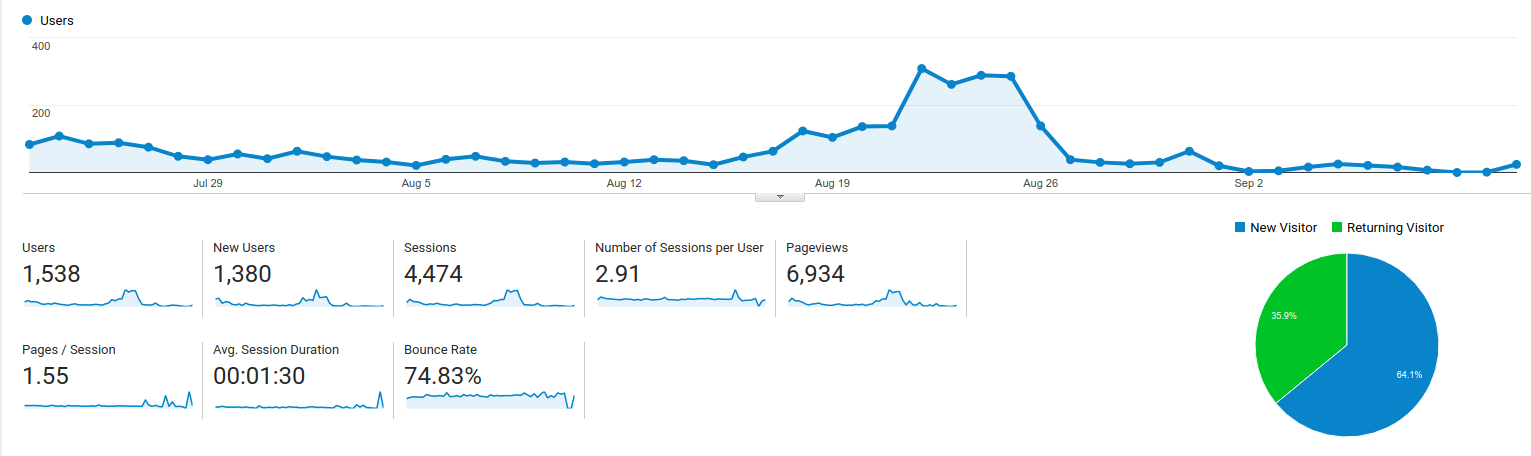
\includegraphics[width=\textwidth]{citadel_1.png}
                \caption{Current semester\label{fig:fig1}}    
            \end{subfigure}
            \vskip\baselineskip
            \begin{subfigure}[ht]{0.9\textwidth}   
                \centering 
                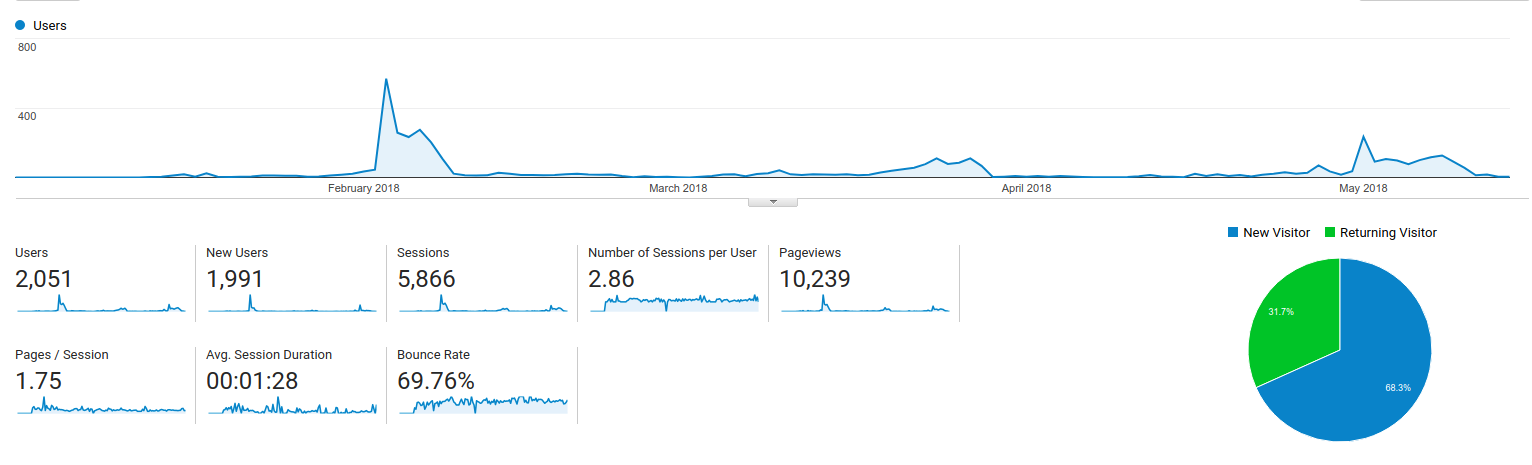
\includegraphics[width=\textwidth]{citadel_2.png}
                \caption{Last semester\label{fig:fig2}}
            \end{subfigure}
            \caption{StudyPortal User analytics \label{fig:study}}
        \end{figure*}
    
    
        \item Yearbook: We tracked the users that were using our portal. See
        \cref{fig:year} for reference.
        \begin{figure*}
            \centering
            \begin{subfigure}[ht]{0.9\textwidth}
                \centering
                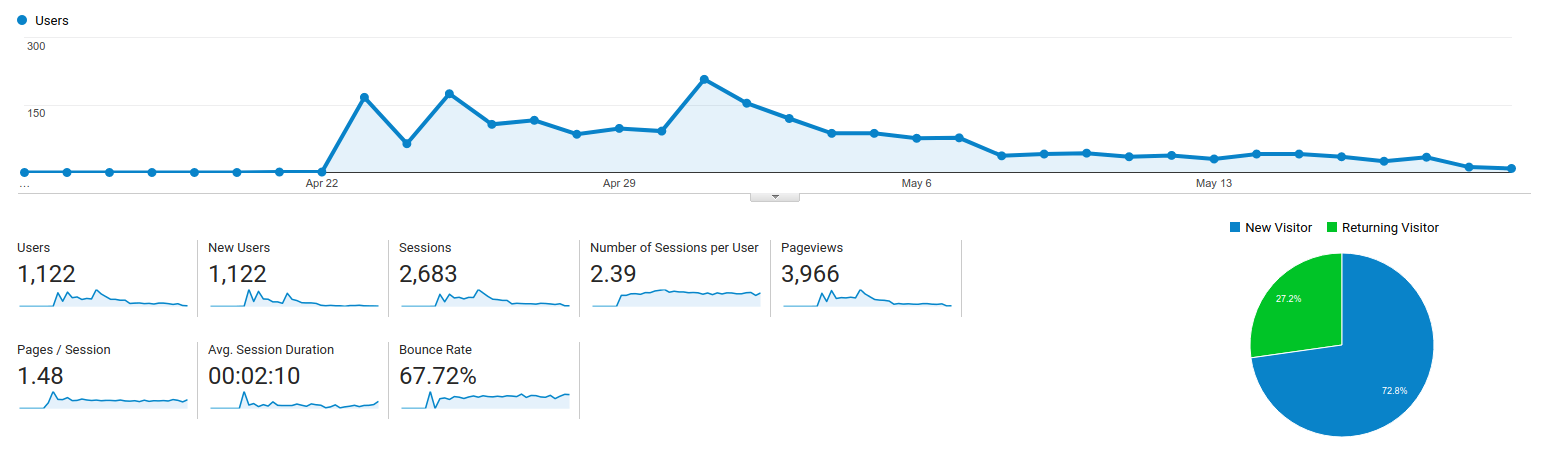
\includegraphics[width=\textwidth]{yearbook.png}
                \caption{Current semester\label{fig:fig3}}    
            \end{subfigure}
            \caption{Yearbook User analytics \label{fig:year}}
        \end{figure*}
    
        \item CampusBot: CampusBot is a chatbot, which we had deployed on facebook messenger. People use it to get details about all sorts of things happening at IITD. It will be integrated into IITD App later.
        \item DevClub lectures: We take lectures on technologies like Web Development, Android Development, Git, Design Practices etc. This helps the first year students to get an idea about different technologies and they can better find their passion.
        \item Winter Assignments: We floated some simple assignments last winter that helped students practice different technologies and frameworks they had learnt throughout the year as part of our lecture series. We were ourselves surprised by the amount of submissions we received.
        \item Most importantly, people see us as a group they can lean on to when they want some tech related help. People ask us everyday to build something for them, but due to lack of more members and funds, we cannot help everyone. We hope that one day our club is big enough to satisfy everyone's needs.
    \end{enumerate}
    \section{Budget}
    \subsection{Sponsorships}
    Sponsorship permission is required to collaborate with tech giants like Microsoft and Google which will enable us to organize technical events on a larger scale. 
    
    \subsection{Budget requirements}
    
    \begin{table}[h!]
    \centering
    \begin{tabular}{|c|c|c|}
        \toprule
        Details                                 &   Quantity            &   Amount (in Rs.) \\
        \midrule
        Event Publicity Costs                   &   6 Planned Events    &   2,500.00         \\
        % Event Miscellaneous costs                      &   6 Planned Events    &   10,000.00          \\
        Hackathon Prizes (1 Hackathon Per Year) &   8 - 9               &   8,000.00         \\
        Domain Subscription Fee                 &   1                   &   1,000.00         \\
        AWS Server Costs                        &   1                   &   15,000.00          \\
        Google Play Console Subscription        &   1                   &   1,800.00         \\
        Internal Hackathon and Events           &   4                   &   15,000.00         \\
        \hline
        \textsc{Total Projected Cost(Year 1)} & & \fbox{43,300.00} \\
        \bottomrule                
        \end{tabular}
    \end{table}
    
    \begin{itemize}
        \item \textbf{Event Publicity Costs} :- A fixed amount of budget is needed to publicize events using posters which cost Rs. 20 per piece. Considering 6 planned events per year which include 1 orientation, 1 Hackathon and 4 lectures with an average of 20 posters per event, a budget of roughly Rs. 2500 is needed for event publicity.
        \item \textbf{Hackathon Prizes} :- The hackathons organized once a year will have prizes for top 3 teams which can have upto 3 members. The average cost of prizes will be Rs. 900. In case of less number of members in teams, the extra amount will be distributed as runner up prizes to upto 2 extra teams.
        \item \textbf{Domain Subscription Fee} :- An amount of Rs. 1000 is needed for the yearly fee of the domain www.devclub.in which provides external access to DevClub's website.
        \item \textbf{AWS Server Costs} :- The annual server cost for the projects hosted at www.devclub.in is Rs. 15000. This is computed at the pricing of 0.02 USD per hour. This amounts to $0.023*365*24 = 201.48$ USD $= 15,000$ INR
        \item \textbf{Google Play Console Subscription} :- This is required to publish the IITD App which is being developed for android applications and will be freely available for the use of all students. (Refer Ongoing Projects in Section 2.1 for more details).
        \item \textbf{Internal Hackathon and Events} :- We organize hackathons and internal club events to encourage learning about new technologies. These events also include a team dinner once a year (Rs. 7,500). The projected total cost of these events comes out to be Rs. 15,000.
        
    \end{itemize}
    \end{document}